\setchapterpreamble[u]{\margintoc}
\chapter{Introduction}
\labch{intro}

\section{The Main Ideas}

Many modern printed textbooks have adopted a layout with prominent 
margins where small figures, tables, remarks and just about everything 
else can be displayed. Arguably, this layout helps to organise the 
	discussion by separating the main text from the ancillary material, 
	which at the same time is very close to the point in the text where 
	it is referenced.

This document does not aim to be an apology of wide margins, for there 
are many better suited authors for this task; the purpose of all these 
words is just to fill the space so that the reader can see how a book 
written with the kaobook class looks like. Meanwhile, I shall also try 
to illustrate the features of the class.

The main ideas behind kaobook come from this 
\href{https://3d.bk.tudelft.nl/ken/en/2016/04/17/a-1.5-column-layout-in-latex.html}{blog 
	post}, and actually the name of the class is dedicated to the author 
of the post, Ken Arroyo Ohori, which has kindly allowed me to create a 
class based on his thesis. Therefore, if you want to know more reasons 
to prefer a 1.5-column layout for your books, be sure to read his blog 
post.

Another source of inspiration, as you may have noticed, is the 
\href{https://github.com/Tufte-LaTeX/tufte-latex}{Tufte-Latex Class}. 
The fact that the design is similar is due to the fact that it is very 
difficult to improve something wich is already so good. However, I like 
to think that this class is more flexible than Tufte-Latex. For 
instance, I have tried to use only standard packages and to implement as 
little as possible from scratch;\sidenote{This also means that 
understanding and contributing to the class development is made easier. 
Indeed, many things still need to be improved, so if you are interested, 
check out the repository on github!} therefore, it should be pretty easy 
to customise anything, provided that you read the documentation of the 
package that provides that feature.

In this book I shall illustrate the main features of the class and 
provide information about how to use and change things. Let us get 
started.

\section{What This Class Does}
\labsec{does}

The \Class{kaobook} class focuses more about the document structure than 
about the style. Indeed, it is a well-known \LaTeX\xspace principle that 
structure and style should be separated as much as possible (see also 
\vrefsec{doesnot}). This means that this class will only provide 
commands, environments and in general, the opportunity to do things, 
which the user may or may not use. Actually, some stylistic matters are 
embedded in the class, but the user is able to customise them with ease.

The main features are the following:

\begin{description}
	\item[Page Layout] The text width is reduced to improve readability 
	and make space for the margins, where any sort of elements can be 
	displayed.
	\item[Chapter Headings] As opposed to Tufte-Latex, we provide a 
	variety of chapter headings among which to choose; examples will be 
	seen in later chapters.
	\item[Page Headers] They span the whole page, margins included, and, 
	in twoside mode, display alternatively the chapter and the section 
	name.\sidenote[][-2mm]{This is another departure from Tufte's 
	design.}
	\item[Matters] The commands \Command{frontmatter}, 
	\Command{mainmatter} and \Command{backmatter} have been redefined in 
	order to have automatically wide margins in the main matter, and 
	narrow margins in the front and back matters. However, the page 
	style can be changed at any moment, even in the middle of the 
	document.
	\item[Margin text] We provide commands \Command{sidenote} and 
	\Command{marginnote} to put text in the 
	margins.\sidenote[][-2mm]{Sidenotes (like this!) are numbered while 
	marginnotes are not}
	\item[Margin figs/tabs] A couple of useful environments is 
	\Environment{marginfigure} and \Environment{margintable}, which, not 
	surprisingly, allow you to put figures and tables in the margins 
	(\cfr \reffig{marginmonalisa}).
	\item[Margin toc] Finally, since we have wide margins, why don't add 
	a little table of contents in them? See \Command{margintoc} for 
	that.
	\item[Hyperref] \Package{hyperref} is loaded and by default we try 
	to add bookmarks in a sensible way; in particular, the bookmarks 
	levels are automatically reset at \Command{appendix} and 
	\Command{backmatter}. Moreover, we also provide a small package to 
	ease the hyperreferencing of other parts of the text.
	\item[Bibliography] We want the reader to be able to know what has 
	been cited without having to go to the end of the document every 
	time, so citations go in the margins as well as at the end, as in 
	Tufte-Latex. Unlike that class, however, you are free to customise 
	the citations as you wish.
\end{description}

\begin{marginfigure}[-5.5cm]
	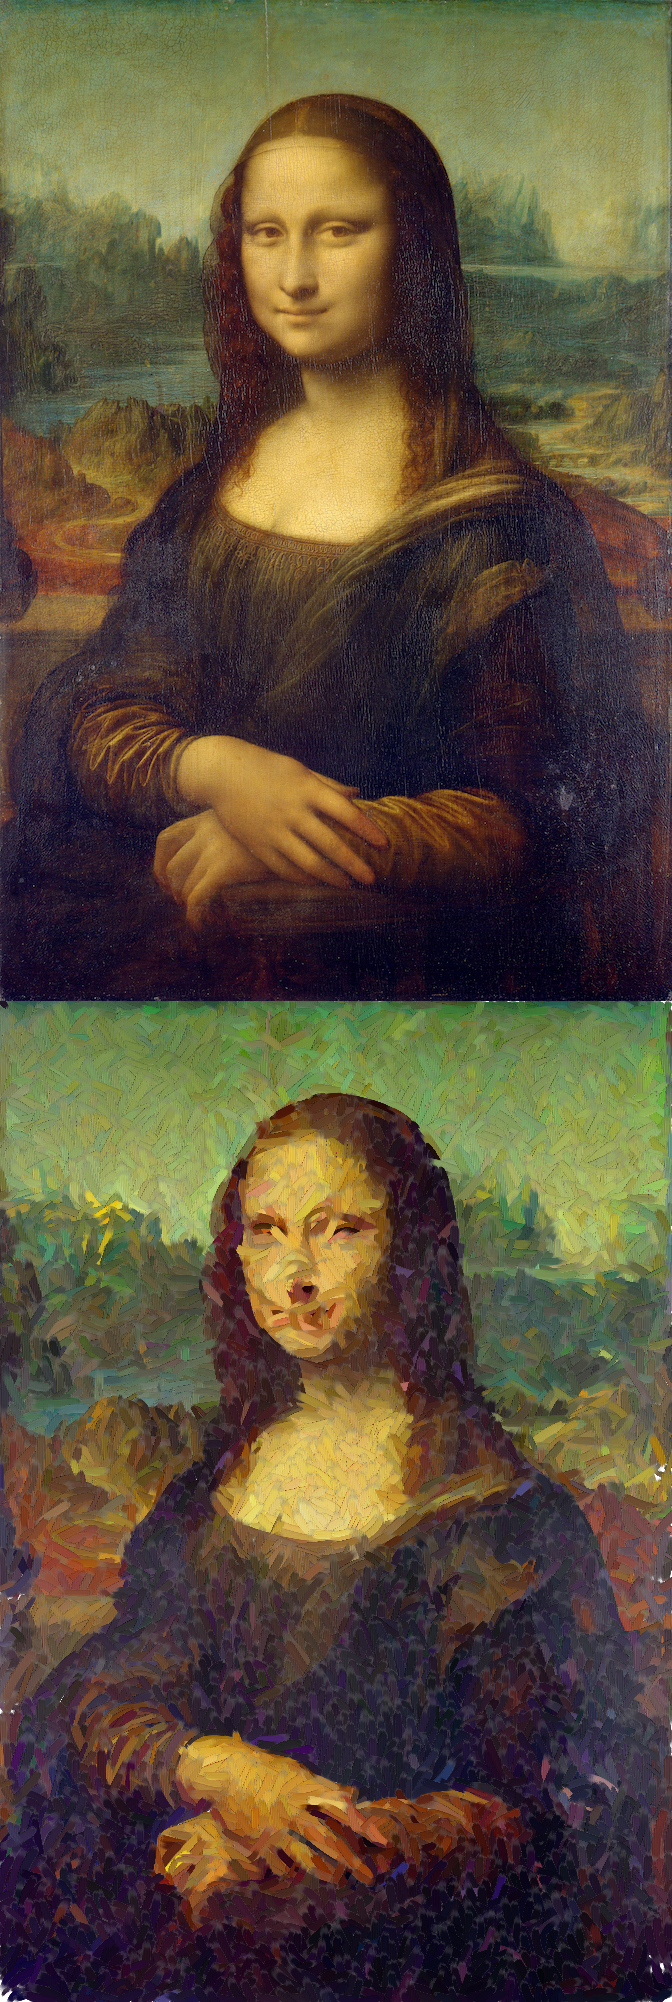
\includegraphics{monalisa}
	\caption[The Mona Lisa]{The Mona Lisa.\\ 
	\url{https://commons.wikimedia.org/wiki/File:Mona_Lisa,_by_Leonardo_da_Vinci,_from_C2RMF_retouched.jpg}}
	\labfig{marginmonalisa}
\end{marginfigure}

The order of the title pages, table of contents and preface can be 
easily changed, as in any \LaTeX\ document. In addition, the class is 
based on \KOMAScript's \Class{scrbook}, therefore it inherits all the 
goodies of that.

\section{What This Class Does Not Do}
\labsec{doesnot}

As anticipated, further customisation of the book is left to the user. 
Indeed, every book may have sidenotes, margin figures and so on, but 
each book will have its own fonts, toc style, special environments and 
so on. For this reason, in addition to the class, we provide only 
sensible defaults, but if these features are not needed, they can be 
left out. These special packages are located in the \Path{style} 
directory, which is organised as follows:

\begin{description}
	\item[kao.sty] This package contains the most important definitions 
	of macros and specifications of page layout. It is the heart of the 
	\Class{kaobook}.
	\item[kaobiblio.sty] Contains commands to add citations and 
	customise the bibliography.
	\item[packages.sty] Loads additional packages to decorate the 
	writing with special contents (for instance, the \Package{listing} 
	package is loaded here as it is not required in every book). There 
	are also defined some useful commands to print the same words always 
	in the same way, \eg latin words in italics or \Package{packages} in 
	verbatim.
	\item[kaorefs.sty] Some useful commands to manage labeling and 
	referencing, again to ensure that the same elements are referenced 
	always in a consistent way.
	\item[environments.sty] Provides special environments, like boxes. 
	Both simple and complex environments are available; by complex we 
	mean that they are endowed with a counter, floating and can be put 
	in a special table of contents.\sidenote[][-2mm]{See 
	\vrefch{mathematics} for some examples.}
	\item[theorems.sty] The style of mathematical environments. 
	Acutally, there are two such packages: one is for plain theorems, 
	\ie the theorems are printed in plain text; the other uses 
	\Package{mdframed} to draw a box around theorems. You can plug the 
	most appropriate style into its document.
\end{description}

\marginnote[2mm]{The audacious users might feel tempted to edit some of 
these packages. I'd be immensely happy if they sent me examples of what 
they have been able to do!}

In the rest of the book, I shall assume that the reader is not a novice 
in the use of \LaTeX, and refer to the documentation of the packages 
used in this class for things that are already explained there. 
Moreover, I assume that the reader is willing to make minor edits to the 
provided packages for styles, environments and commands, if he or she 
does not like the default settings.

\section{How to Use This Class}

Either if you are using the template from 
\href{https://latextemplates.org/template/kaobook}{latextemplates}, or if 
you cloned the GitHub 
\href{https://www.github.com/fmarotta/kaobook}{repository}, there are 
infinite ways to use the \Class{kaobook} class in practice. To get started,
find the \Path{main.tex} file which I used to write this book, and edit it; this 
will probably involve a lot of text-deleting, copying-and-pasting, and rewriting.

To compile the document, assuming that its name is \Path{main.tex}, you 
will have to run the following sequence of commands:

\begin{lstlisting}[style=kaolstplain,linewidth=1.5\textwidth]
pdflatex main # Compile template
makeindex main.nlo -s nomencl.ist -o main.nls # Compile nomenclature
makeindex main # Compile index
biber main # Compile bibliography
makeglossaries main # Compile glossary
pdflatex main # Compile template again
pdflatex main # Compile template again
\end{lstlisting}

You may need to compile the template some more times in order for some 
errors to disappear. For any support requests, please ask a question on 
\url{tex.stackexchange.org} with the tag \enquote{kaobook}, open an 
issue on GitHub, or contact the author via e-mail.
